% ---- SECTION CONCEPTION ET IMPLÉMENTATION ----

% -------------------------------------------------------
\section{Environnement de conception et de développement}
Pour mener à bien ce projet mécatronique, plusieurs outils professionnels de conception et de développement ont été mobilisés. Ils permettent de garantir la précision des modèles et l'interopérabilité des données.

\subsection{Conception mécanique et électronique}
\begin{itemize}
    \item \textbf{SolidWorks (Dassault Systèmes) :} Utilisé pour la modélisation 3D intégrale du prototype, les simulations d'assemblage et la génération des mises en plan techniques. C'est le standard industriel pour la conception de systèmes mécaniques complexes.
    \item \textbf{KiCad EDA :} Suite logicielle open-source retenue pour la saisie schématique et le routage du PCB. Sa flexibilité et sa gratuité en font un outil idéal pour le prototypage rapide en milieu académique et professionnel.
\end{itemize}

\subsection{Développement logiciel}
\begin{itemize}
    \item \textbf{Arduino IDE :} Utilisé pour le codage, la compilation et le téléversement du firmware sur l'ESP32. Sa vaste bibliothèque de pilotes facilite l'interfaçage des capteurs et la gestion du WiFi.
    \item \textbf{VS Code (Visual Studio Code) :} Retenu pour le développement du tableau de bord Internet des objets (HTML/JS) en raison de sa gestion avancée du versionnement (Git) et de son écosystème d'extensions.
\end{itemize}

\begin{figure}[H]
    \centering
    % Première ligne : Conception
    \begin{subfigure}[b]{0.45\textwidth}
        \centering
        
\includegraphics[height=3cm]{images/logo_solidwork.png}
        \caption{SolidWorks (CAO)}
    \end{subfigure}
    \hfill
    \begin{subfigure}[b]{0.45\textwidth}
        \centering
        
\includegraphics[height=3cm]{images/logo_kicad.png}
        \caption{KiCad (EDA)}
    \end{subfigure}
    
    \vspace{0.8cm}
    
    % Deuxième ligne : Développement
    \begin{subfigure}[b]{0.45\textwidth}
        \centering
        
\includegraphics[height=3cm]{images/logo_arduino.png}
        \caption{Arduino IDE (Firmware)}
    \end{subfigure}
    \hfill
    \begin{subfigure}[b]{0.45\textwidth}
        \centering
        
\includegraphics[height=3cm]{images/Visual-Studio-Code-logo.png}
        \caption{VS Code (Tableau de bord IoT)}
    \end{subfigure}
    \caption{Écosystème logiciel utilisé pour le projet SMART-SOJA}
    \label{fig:logos_logiciels}
\end{figure}
\FloatBarrier

\section{Conception électronique : le circuit imprimé (PCB)}

Le schéma électronique global, regroupant l'ensemble des blocs fonctionnels, est consultable en \textbf{Annexe \ref{annexe:schema_global}}.

\subsection{Segmentation fonctionnelle de la conception}
Pour garantir une maintenance aisée et minimiser les interférences électromagnétiques (EMI) entre signaux de puissance et de commande, la conception est segmentée en cinq blocs fonctionnels dès la saisie schématique :

\begin{enumerate}
    \item \textbf{Zone Alimentation (Figure \ref{fig:zone_alim}) :} Régulateur Buck \textbf{LM2596} générant un rail 5~V / 2~A depuis la source 12~V. La logique 3,3~V est assurée par le régulateur interne de l'ESP32.
    \begin{figure}[H]
        \centering
        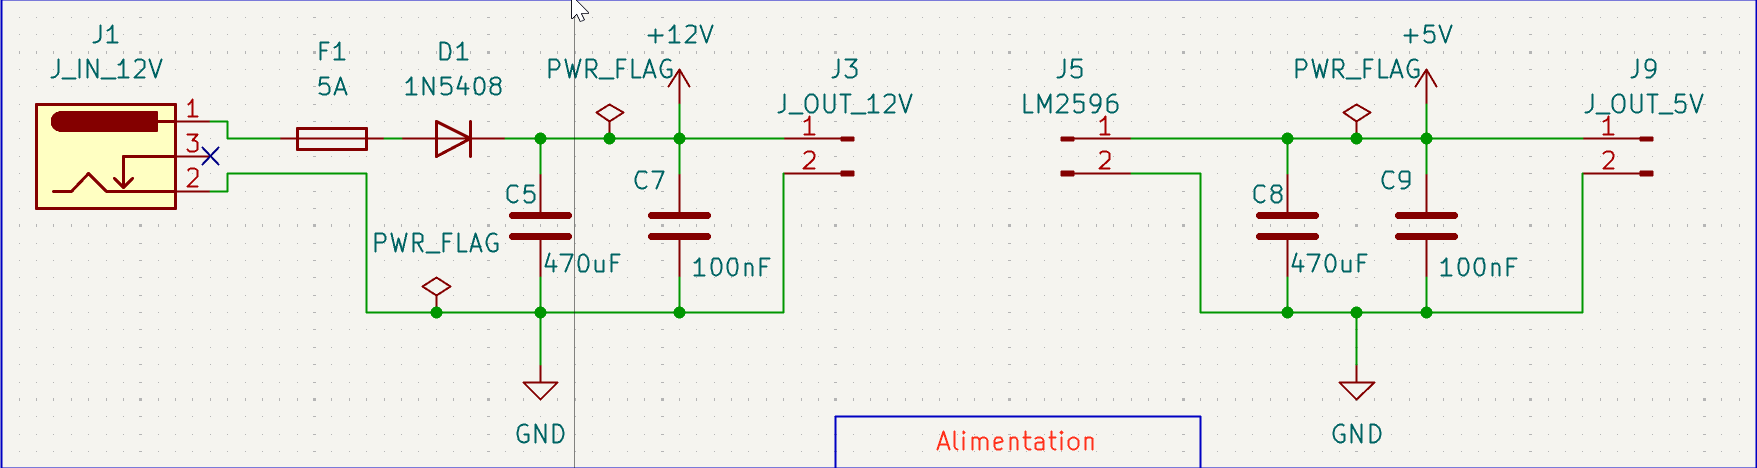
\includegraphics[width=0.55\textwidth]{images/image_circuit_zone-alimentation.PNG}
        \caption{Zone d'alimentation multi-tensions}
        \label{fig:zone_alim}
    \end{figure}

    \item \textbf{Zone ESP32 (Figure \ref{fig:zone_esp32}) :} L'affectation des broches a été optimisée pour éviter les conflits avec les \textit{strapping pins} (GPIO 0, 2, 12, 15) critiques au démarrage.
    \begin{figure}[H]
        \centering
        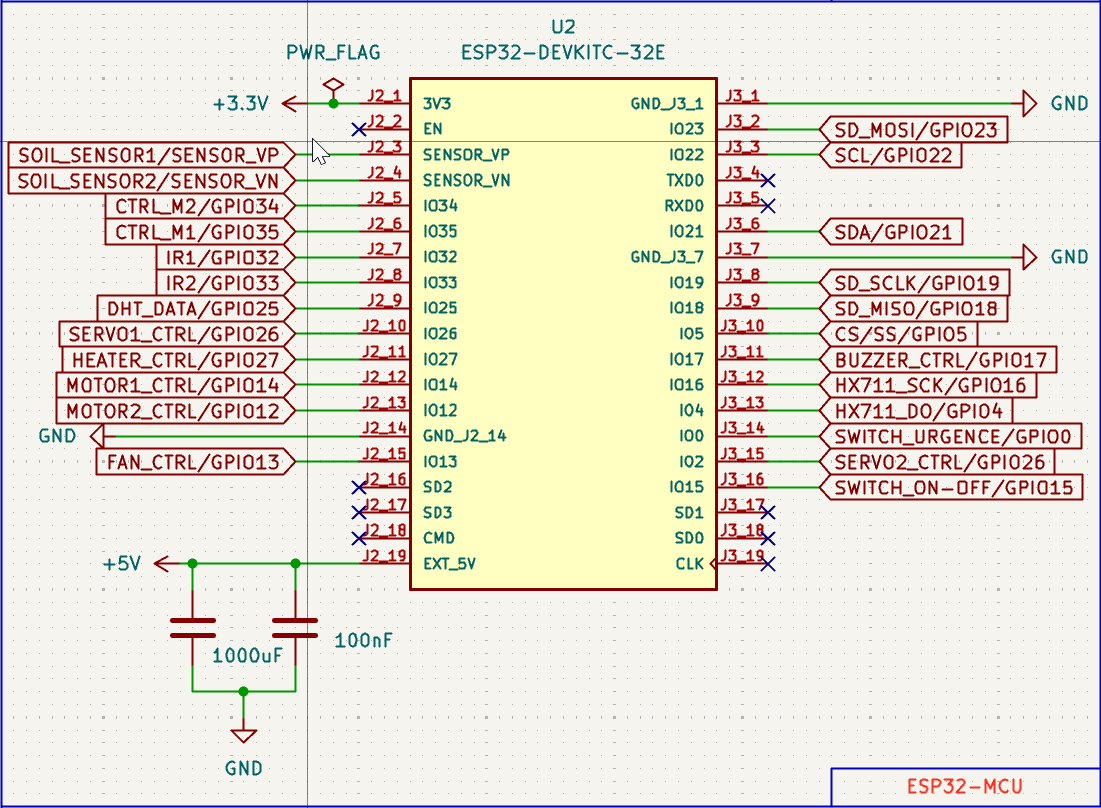
\includegraphics[width=0.55\textwidth]{images/image_circuit_zone-esp32.PNG}
        \caption{Unité de traitement centrale ESP32}
        \label{fig:zone_esp32}
    \end{figure}

    \item \textbf{Zone Puissance (Figure \ref{fig:zone_act}) :} Chaque canal MOSFET IRLZ44N intègre une résistance de grille de 220~$\Omega$, une résistance de rappel pull-down de 10~k$\Omega$ et une diode de roue libre \textbf{1N5408} contre les retours inductifs des moteurs.
    \begin{figure}[H]
        \centering
        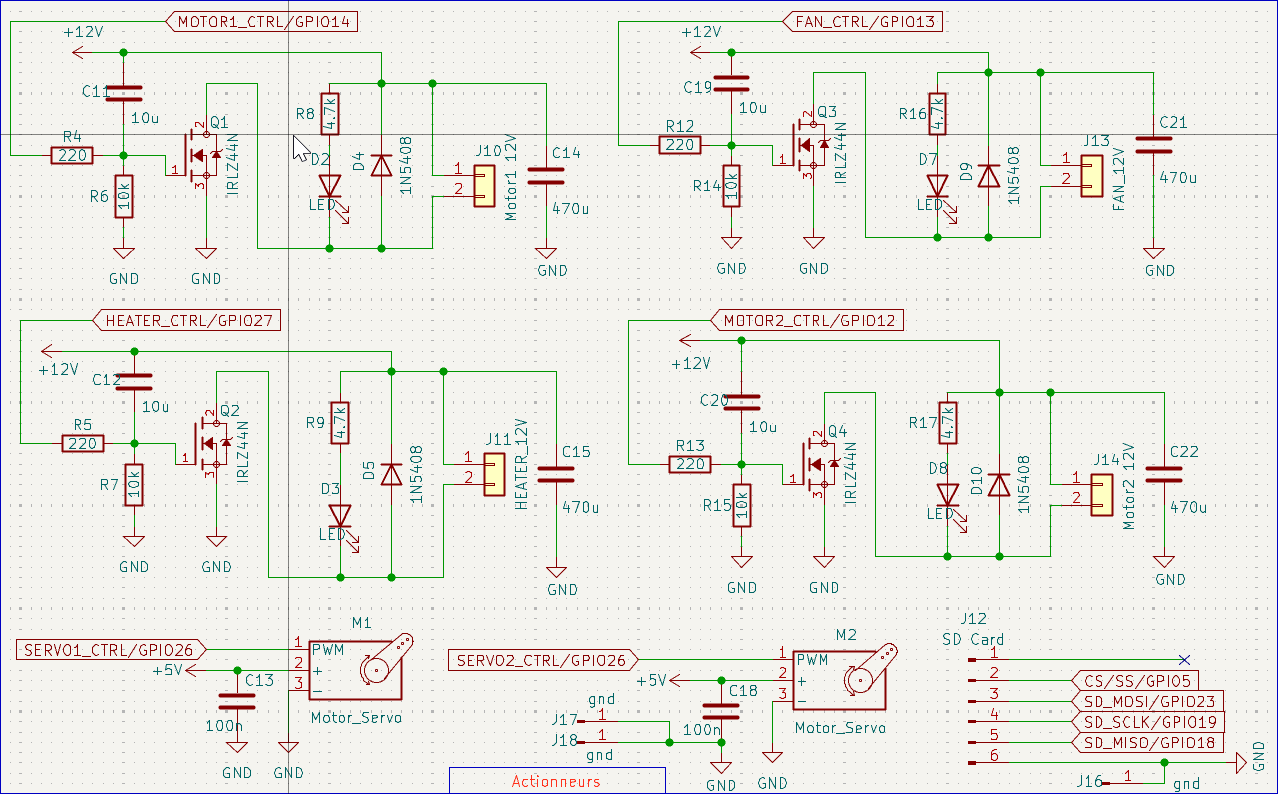
\includegraphics[width=0.55\textwidth]{images/image_circuit_zone-actionneurs.PNG}
        \caption{Étage de puissance avec protections inductives}
        \label{fig:zone_act}
    \end{figure}

    \item \textbf{Zone Acquisition (Figure \ref{fig:zone_cap}) :} Interfaces pour les signaux analogiques (Sondes capacitives sur GPIO 36/39) et numériques (HX711 sur GPIO 25, DHT22, capteurs IR sur GPIO 32/33).
    \begin{figure}[H]
        \centering
        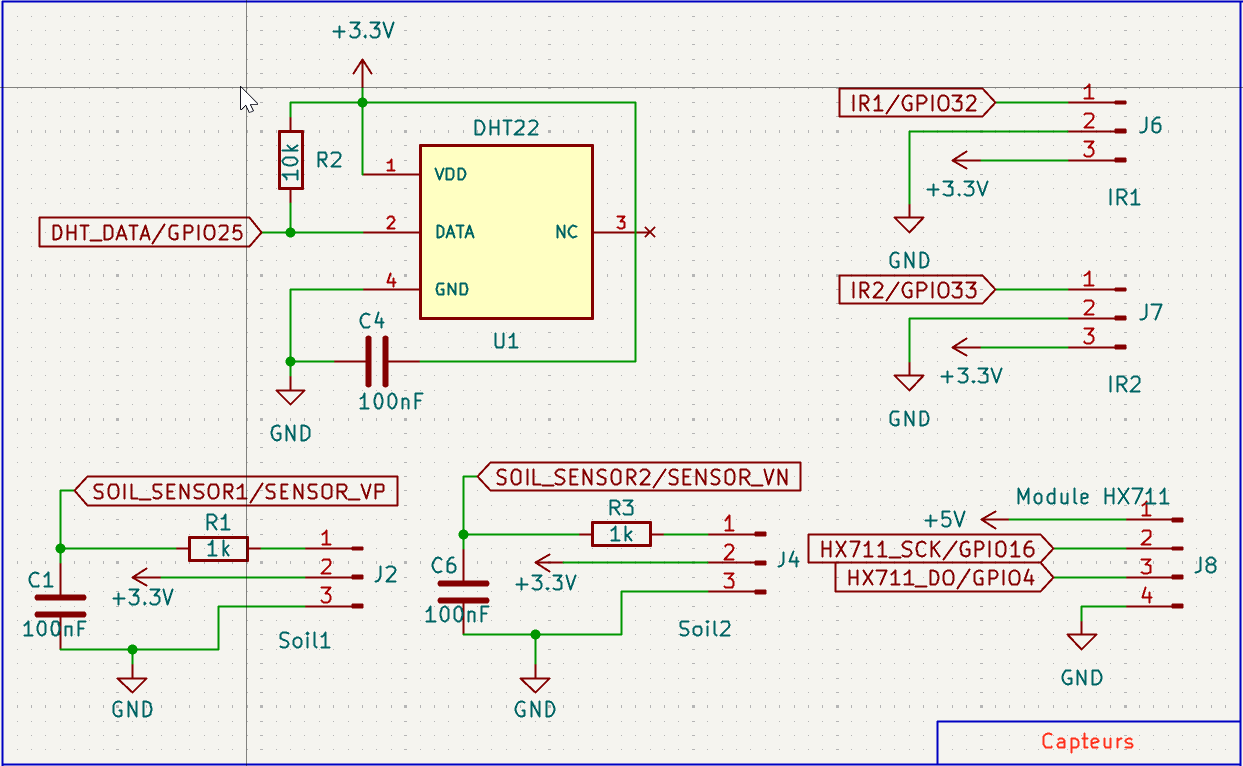
\includegraphics[width=0.55\textwidth]{images/image_circuit_zone-capteurs.PNG}
        \caption{Interface d'acquisition des capteurs}
        \label{fig:zone_cap}
    \end{figure}

    \item \textbf{Zone IHM (Figure \ref{fig:zone_ihm}) :} Gestion du bus I2C (LCD), du bus SPI (carte SD) et des signaux PWM (buzzer, servomoteur, boutons).
    \begin{figure}[H]
        \centering
        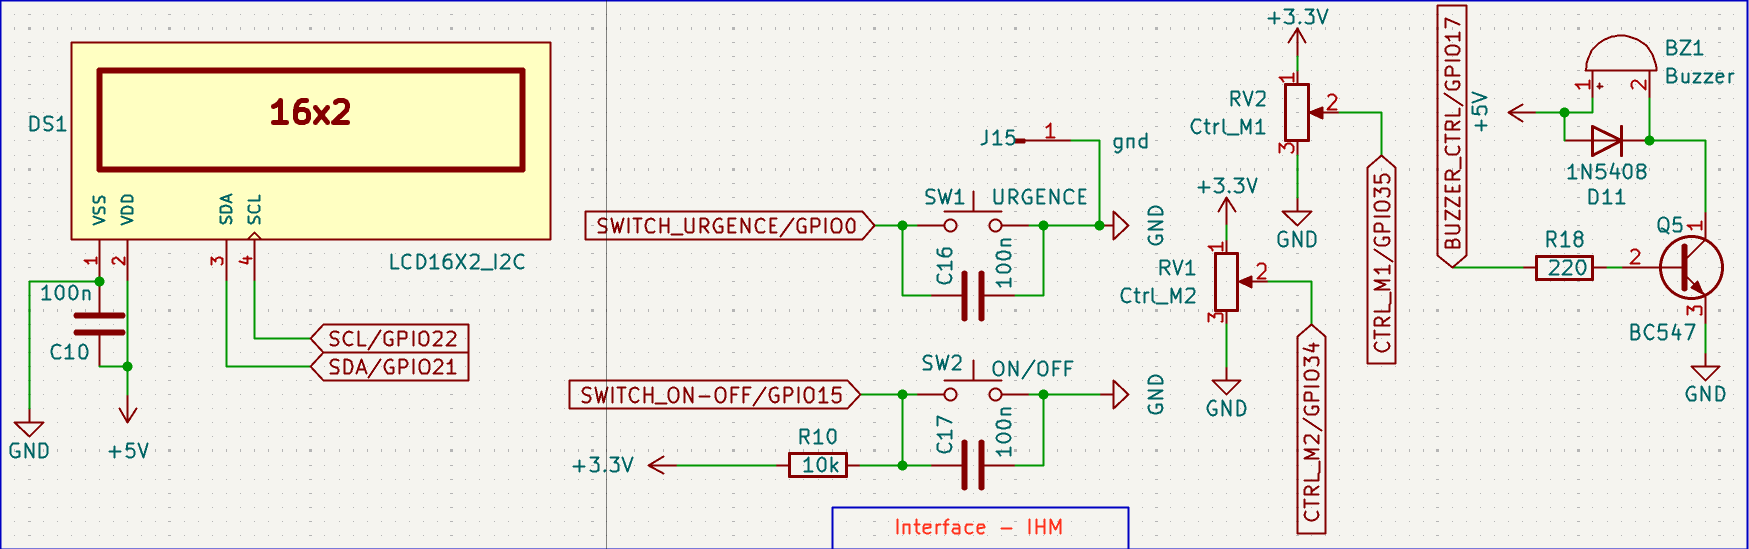
\includegraphics[width=0.55\textwidth]{images/image_circuit_zone-ihm.PNG}
        \caption{Interface Homme-Machine locale}
        \label{fig:zone_ihm}
    \end{figure}
\end{enumerate}
\FloatBarrier

Le routage sous KiCad a été réalisé sur une \textbf{seule couche (Bottom Layer)} pour simplifier la fabrication du prototype. Les pistes de puissance sont dimensionnées à une largeur minimale de \textbf{1~mm} pour supporter les charges inductives sans échauffement. Un plan de masse (Ground Pour) a été généré sur cette face unique pour assurer l'intégrité du signal et limiter les boucles de masse.

La modélisation 3D du PCB a permis de valider l'absence de collision mécanique entre composants volumineux avant fabrication. Les vues détaillées (routage, faces 3D) sont consultables en \textbf{Annexe \ref{annexe:routage_pcb}} et \textbf{Annexe \ref{annexe:vues_3d_pcb}}.

% -------------------------------------------------------
\section{Conception mécanique : architecture modulaire}
% -------------------------------------------------------
La conception mécanique a été réalisée sous \textbf{SolidWorks} selon une architecture modulaire en quatre blocs fonctionnels indépendants (Figure \ref{fig:cad_4blocs}), montés sur un châssis porteur mobile.

\begin{figure}[H]
    \centering
    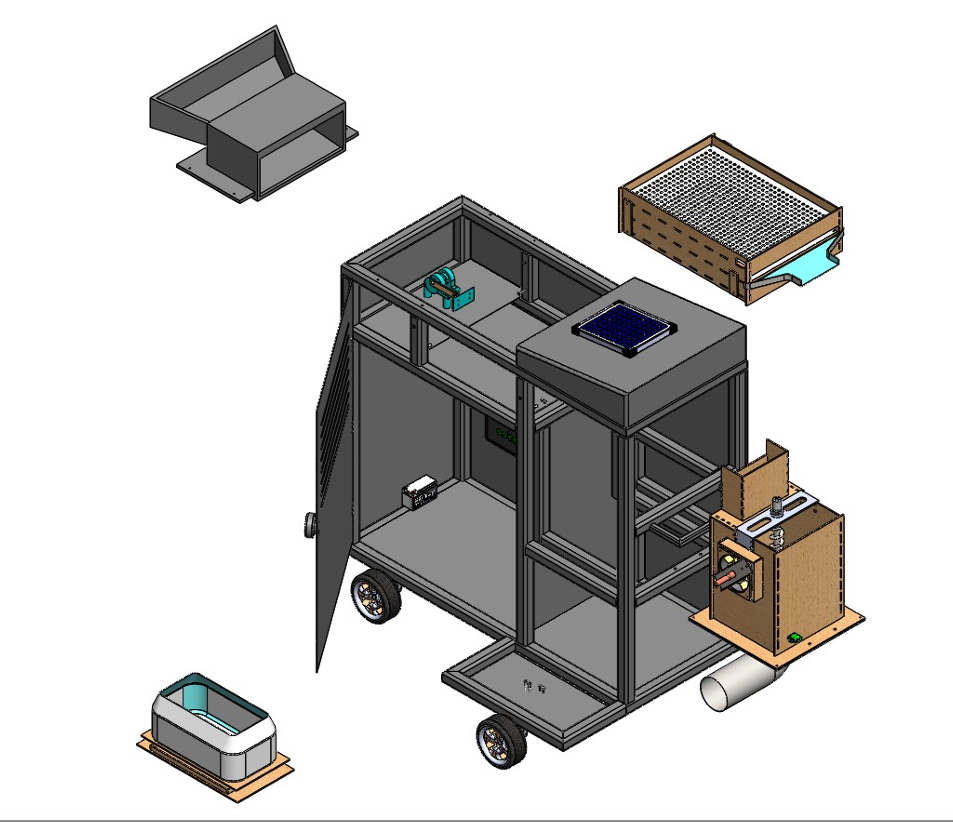
\includegraphics[width=0.85\textwidth]{images/Vue_modulaire_3D.PNG}
    \caption{Architecture modulaire du système SMART-SOJA — Vue d'ensemble CAO}
    \label{fig:cad_4blocs}
\end{figure}
\FloatBarrier


\begin{enumerate}
    \item \textbf{Bloc 1 — Unité d'entrée (Trémie) :} Trémie pyramidale à écoulement gravitaire, pilotée par le servomoteur SG90. Le capteur IR1 confirme la présence de soja avant l'ouverture.

    \item \textbf{Bloc 2 — Unité de nettoyage et vibration :} Deux tamis inox superposés montés sur suspensions élastiques. Le moteur JGA25-370 génère les oscillations via un système poulie-tige de transmission, assurant la séparation granulométrique.

    \item \textbf{Bloc 3 — Unité de séchage et analyse (Figure \ref{fig:sechage_pesee_cad}) :}
    \begin{itemize}
        \item \textbf{Vis sans fin} (type Archimède) : brassage mécanique continu pour un séchage homogène.
        \item \textbf{Ensemble Ventilateur + Résistance Chauffante} : circulation d'air chaud.
        \item \textbf{Boîtiers capteurs} : logements dédiés aux deux sondes capacitives (Soil1/Soil2) et au DHT22.
    \end{itemize}

    \begin{figure}[H]
        \centering
        \begin{subfigure}[b]{0.48\textwidth}
            \centering
            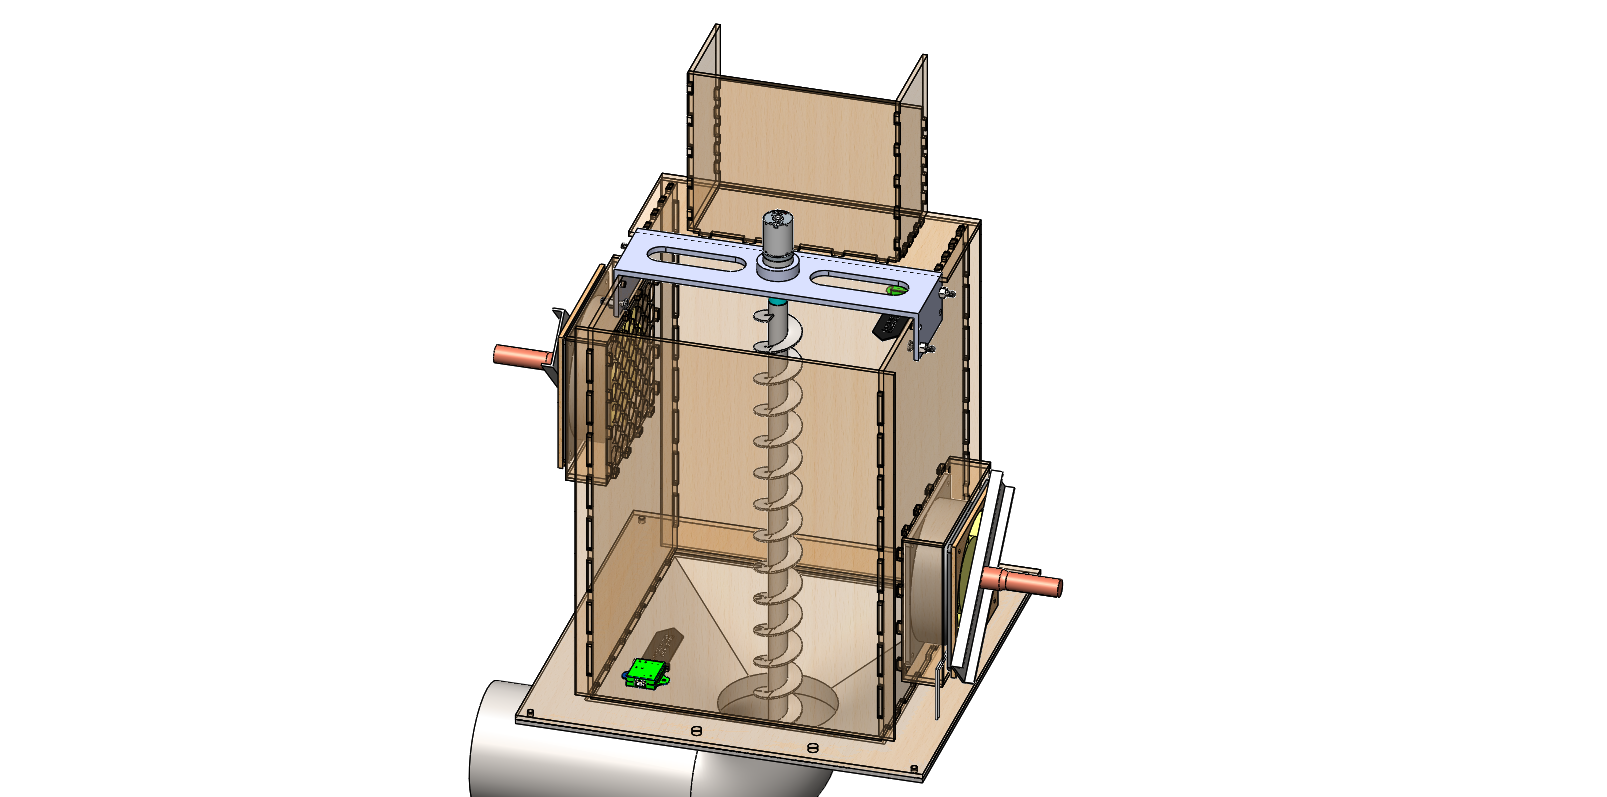
\includegraphics[width=\textwidth]{images/systeme_sechage.PNG}
            \caption{Unité de séchage (Vue 3D)}
        \end{subfigure}
        \hfill
        \begin{subfigure}[b]{0.48\textwidth}
            \centering
            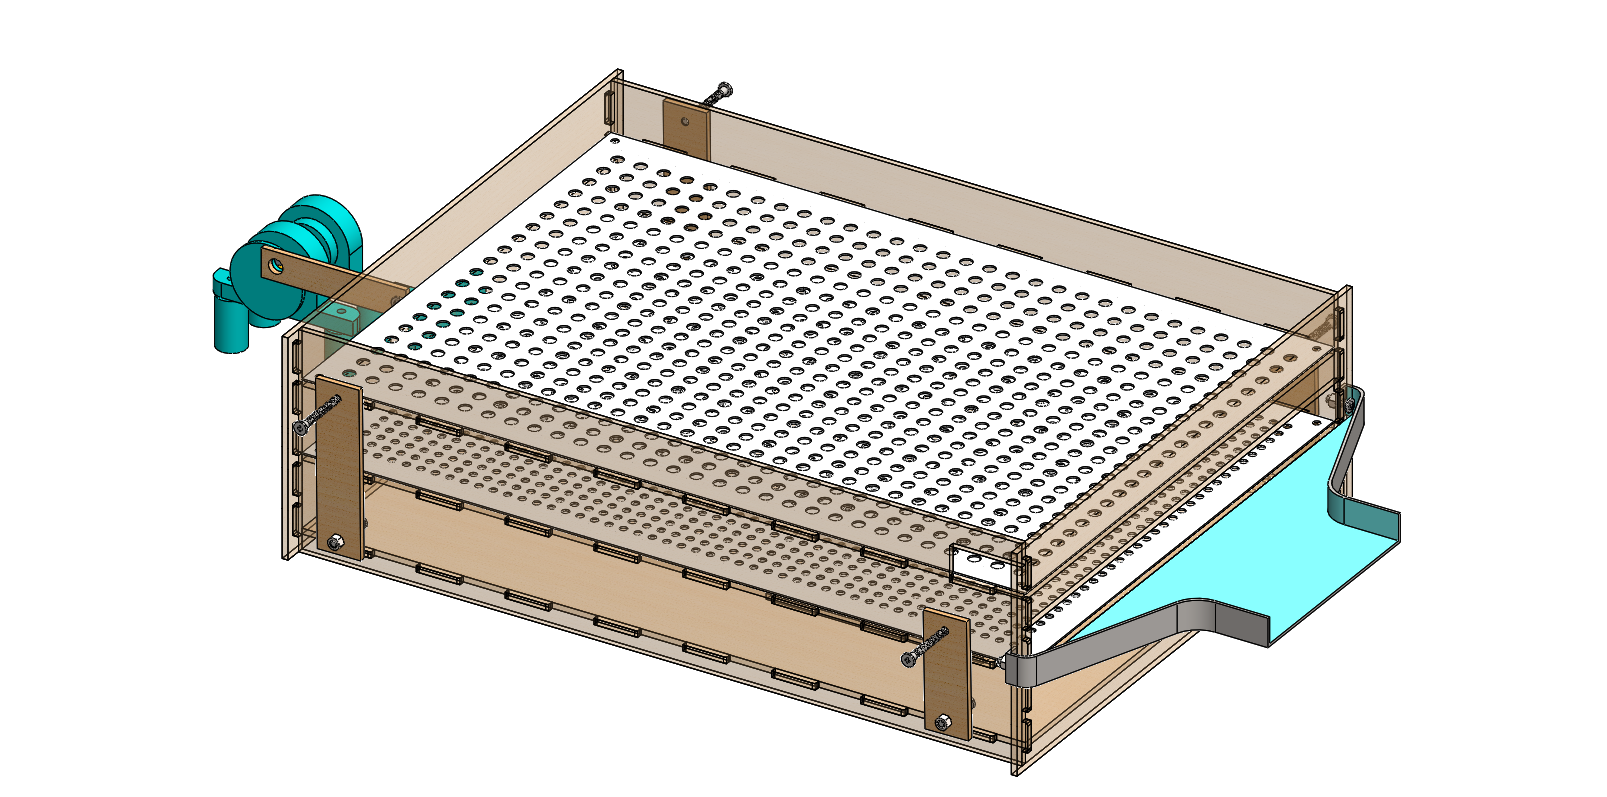
\includegraphics[width=\textwidth]{images/systeme_tami.PNG}
            \caption{Unité de tamisage (Vue 3D)}
        \end{subfigure}
        \caption{Détails des blocs de traitement mécanique sous SolidWorks}
        \label{fig:sechage_pesee_cad}
    \end{figure}
    \FloatBarrier


    \item \textbf{Bloc 4 — Unité de pesée et réception :} Support cellule de charge (Load Cell HX711) avec plateau de réception finale. Le capteur IR2 confirme le retrait du sac en fin de cycle.
\end{enumerate}

\begin{figure}[H]
    \centering
    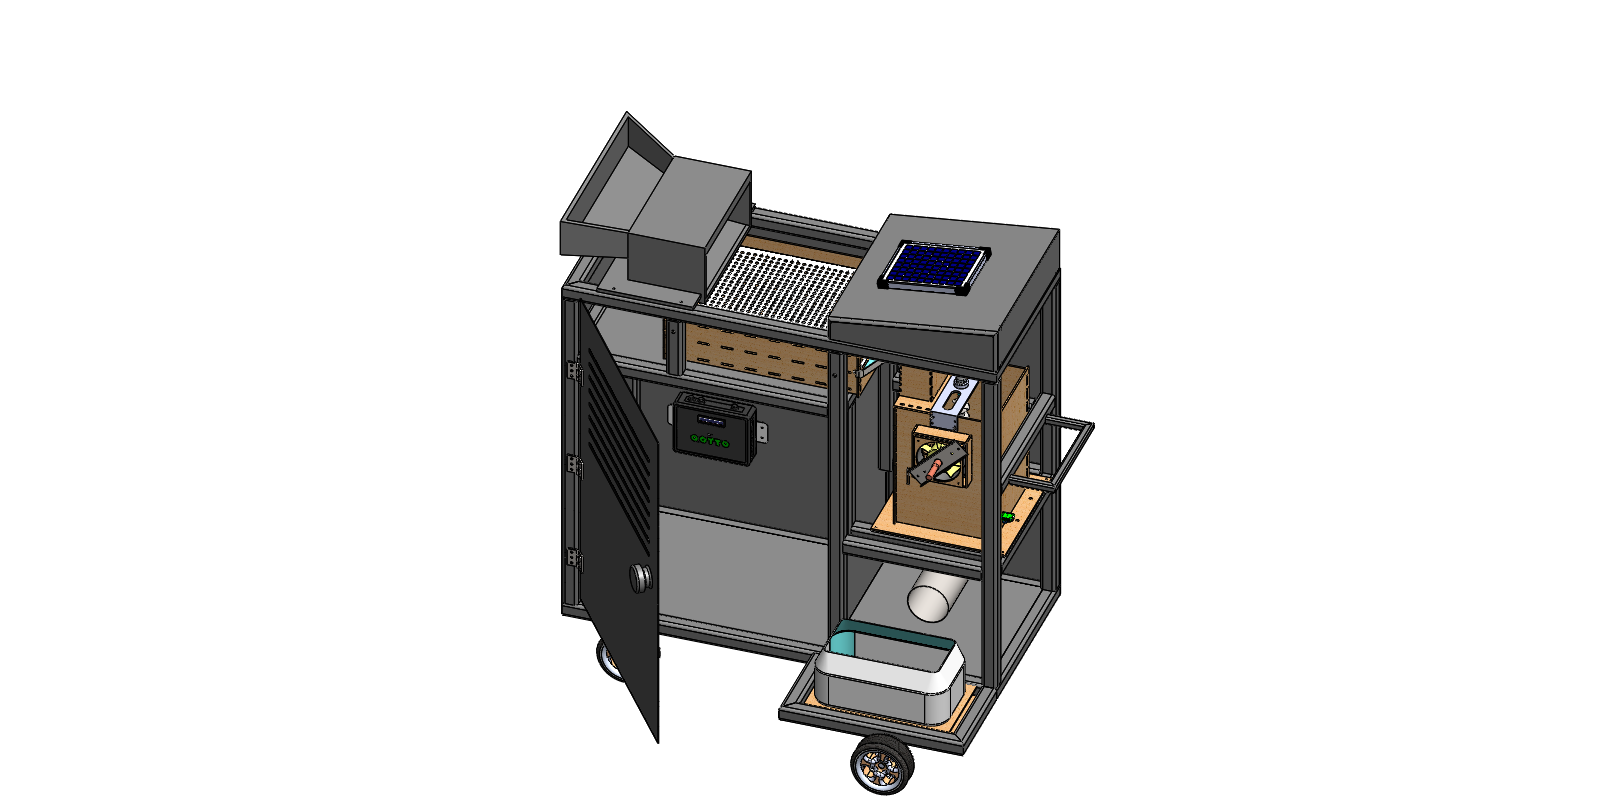
\includegraphics[width=1.02\textwidth]{images/Smart-Soja.PNG}
    \caption{Vue d'ensemble du prototype SMART-SOJA assemblé (SolidWorks)}
    \label{fig:systeme_complet}
\end{figure}
\FloatBarrier

\begin{figure}[H]
    \centering
    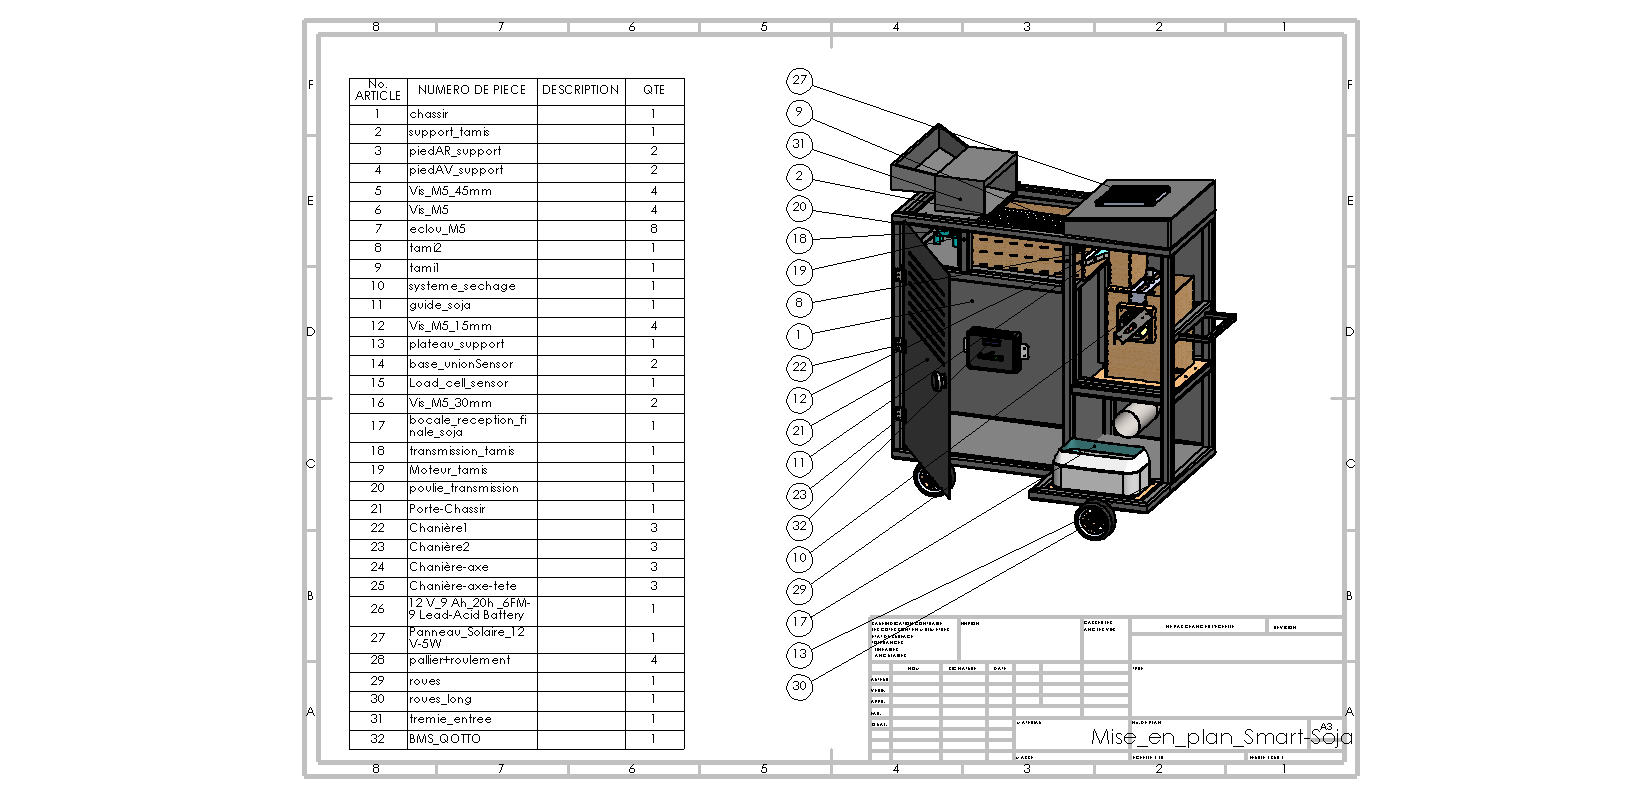
\includegraphics[width=\textwidth]{images/Mise_en_plan_Smart-Soja.PNG}
    \caption{Mise en plan technique et nomenclature (BOM) du châssis}
    \label{fig:mise_en_plan}
\end{figure}
\FloatBarrier

Chaque bloc peut être retiré du châssis sans démonter l'intégralité du système grâce à un système de glissières et connecteurs rapides — facteur clé pour la maintenance en milieu rural isolé.

\subsection{Fabrication et assemblage physique du châssis}
La phase de fabrication mécanique du châssis a nécessité la découpe de panneaux de contreplaqué haute densité aux dimensions précises de la modélisation SolidWorks. Cette opération a été réalisée à l'atelier de \textbf{Sèmè City Open Park} à l'aide d'une scie circulaire sur table (Figure~\ref{fig:decoupe_contreplaque}).

\begin{figure}[H]
    \centering
    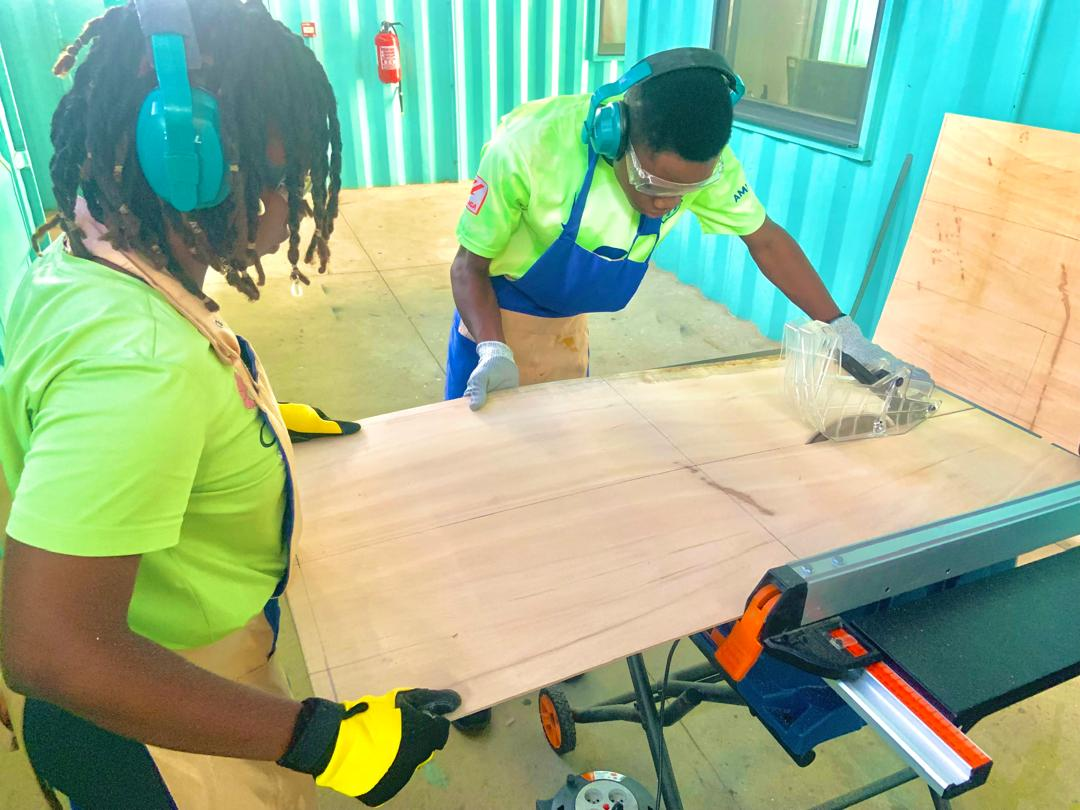
\includegraphics[width=0.55\textwidth]{images/decoupe_plaquet.jpg}
    \caption{Découpe du contreplaqué pour le châssis SMART-SOJA à Sèmè City Open Park}
    \label{fig:decoupe_contreplaque}
\end{figure}
\FloatBarrier

% -------------------------------------------------------
\section{Implémentation du firmware embarqué}
% -------------------------------------------------------
\label{sec:freertos_implementation}

\subsection{Architecture multitâches FreeRTOS}
Le firmware SMART-SOJA implémente \textbf{6 tâches FreeRTOS} ordonnancées selon leur criticité. La communication inter-tâches s'effectue via 5 files de messages (queues) pour un découplage robuste sans conditions de course (Tableau \ref{tab:freertos_tasks}).

\begin{table}[H]
    \caption{Hiérarchie des tâches FreeRTOS du firmware SMART-SOJA}
    \label{tab:freertos_tasks}
    \centering
    \small
    \renewcommand{\arraystretch}{1.8}
    \rowcolors{2}{white}{lightGray}
    \begin{tabularx}{\textwidth}{|L|>{\bfseries}C|C|L|}
        \hline
        \rowcolor{lightGray}
        \textbf{Tâche} & \textbf{Priorité} & \textbf{Cycle} & \textbf{Fonction} \\ \hline
        Task\_Safety    & 4 (MAX)  & 10 ms  & Arrêt d'urgence, surchauffe, timeout — temps réponse $<$ 10 ms. \\ \hline
        Task\_Control   & 3 (HIGH) & 50 ms  & Automate GRAFCET, gestion des transitions d'états. \\ \hline
        Task\_Sensing   & 2 (MED)  & 100 ms & Acquisition DHT22, Soil1/2, HX711 avec filtrage passe-bas. \\ \hline
        Task\_Actuators & 2 (MED)  & 50 ms  & Pilotage PWM moteurs, servo, LEDs. \\ \hline
        Task\_LCD       & 1 (LOW)  & 200 ms & Affichage I2C + lecture potentiomètres (ADC 0--4095 → 0--100\%). \\ \hline
        Task\_MQTT      & 1 (LOW)  & 500 ms & Transmission JSON, Store-and-Forward sur SD si déconnecté. \\ \hline
    \end{tabularx}
\end{table}
\FloatBarrier

Le flux de synchronisation entre tâches est illustré en Figure \ref{fig:arch_freertos} :

\begin{figure}[H]
    \centering
    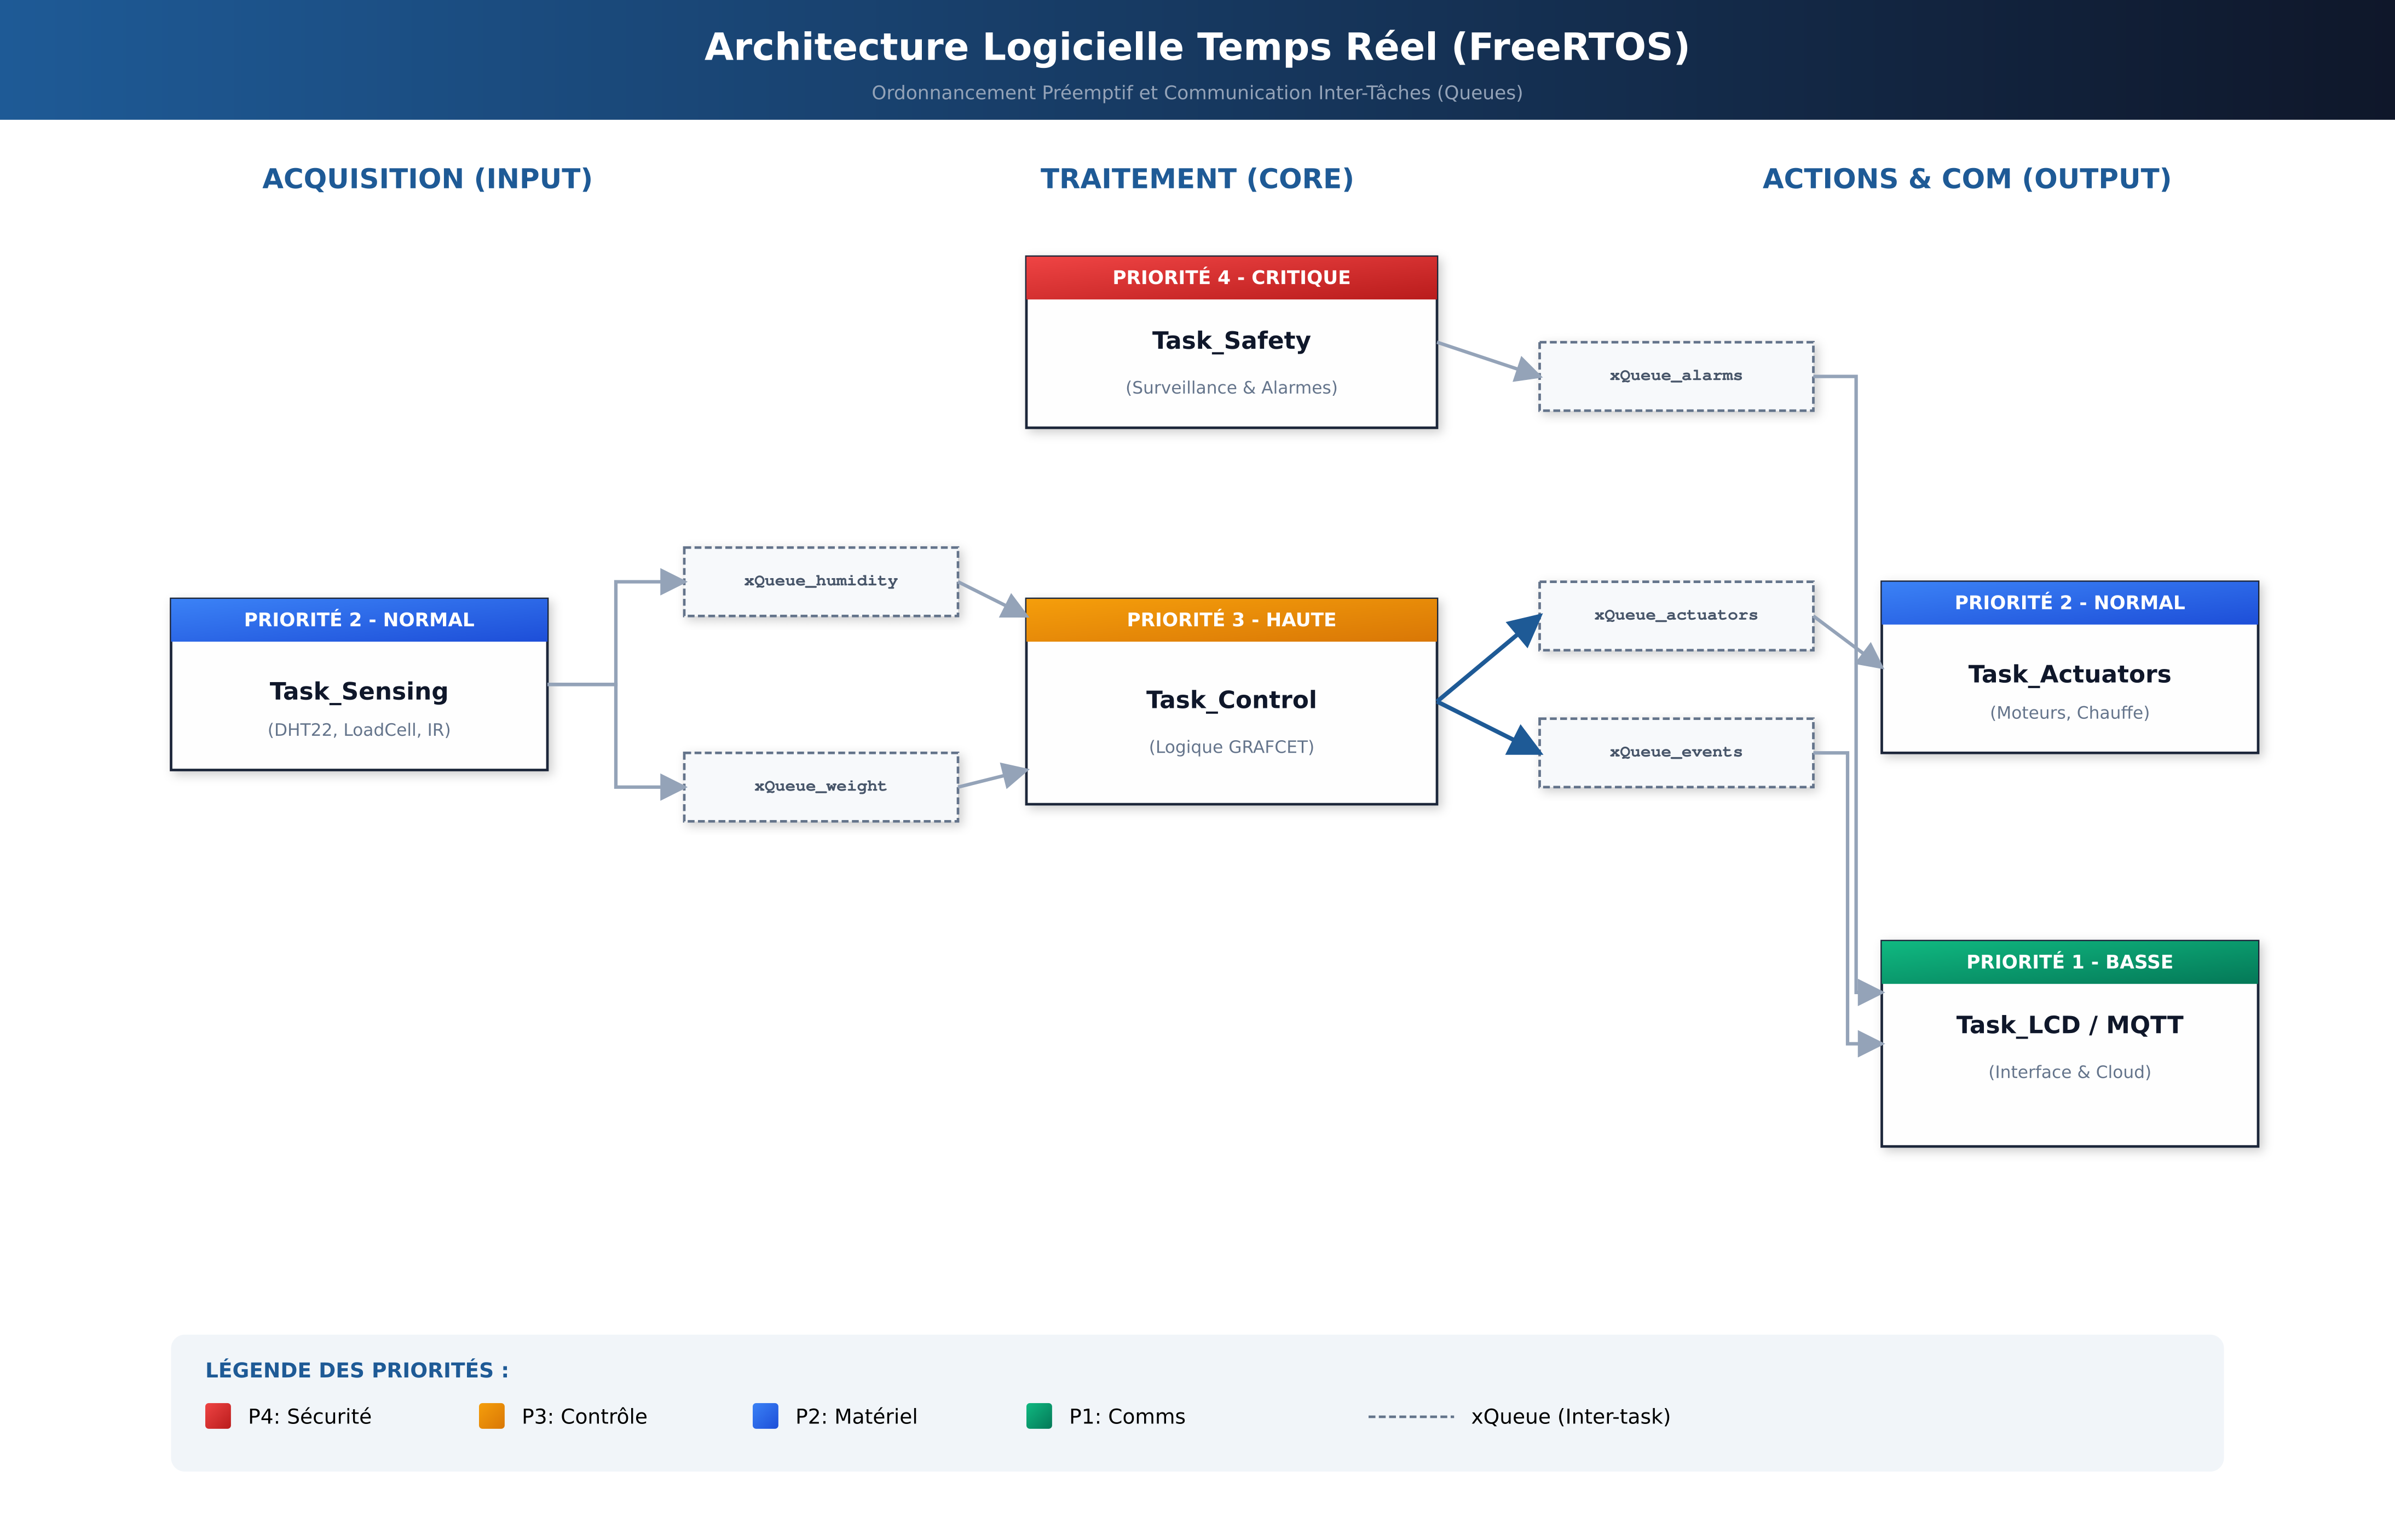
\includegraphics[width=\textwidth]{images/freertos_tasks.png}
    \caption{Diagramme de synchronisation des tâches FreeRTOS — SMART-SOJA}
    \label{fig:arch_freertos}
\end{figure}
\FloatBarrier

\subsection{Sérialisation et format de données (JSON)}
L'échange de données entre l'unité mobile ESP32 et la plateforme web de supervision s'effectue sous forme de messages sérialisés au format JSON. Deux types de trames sont principalement transmis :

\vspace{0.3cm}
\noindent\textbf{1. Trame de télémétrie périodique} (publiée toutes les 5~secondes sur le topic \texttt{smart-soja/telemetry/\{unitId\}}) : elle assure le suivi en temps réel de l'état de fonctionnement du prototype.
\begin{verbatim}
{
  "unitId": "SS-000110",
  "timestamp": 1716633600000,
  "humidity": 12.5,
  "temperature": 31.8,
  "weight": 42.3,
  "ir1": true,
  "ir2": false,
  "mode": "auto",
  "step": 3,
  "alarm": false,
  "controls": {
    "alimentation": false,
    "tamis": true,
    "ventilateur": false,
    "chauffage": true,
    "vis_soja": true,
    "servo_vanne": false
  },
  "battery": 95
}
\end{verbatim}

\vspace{0.3cm}
\noindent\textbf{2. Trame d'archivage de fin de cycle} (publiée sur le topic \texttt{smart-soja/lot\_completed/\{unitId\}} lors de la finalisation du traitement d'un lot) : elle certifie la qualité finale du soja.
\begin{verbatim}
{
  "unitId": "SS-000110",
  "timestamp": 1716633780000,
  "lotId": "LOT-TEST-002",
  "duration_ms": 180000,
  "weight_processed": 5000,
  "humidity_avg": 10.8,
  "temperature_avg": 31.8,
  "steps_completed": 12,
  "quality_score": 95
}
\end{verbatim}
\vspace{0.2cm}

Ce format de \textbf{passeport numérique} constitue la pièce centrale de la traçabilité Internet des objets : il lie chaque sac de soja à ses métriques de qualité certifiées, consultables depuis le tableau de bord web.

% -------------------------------------------------------
\section{Plateforme Internet des objets : tableau de bord de supervision}
% -------------------------------------------------------
La plateforme web \textbf{SMART-SOJA} constitue le centre de supervision et de traçabilité à distance du système. Elle a été développée selon une architecture de type \textbf{SPA} (\textit{Single Page Application}) en utilisant l'outillage moderne \textbf{Vite.js} et du \textbf{JavaScript (Vanilla JS)}. Ce choix garantit une interface utilisateur fluide, réactive et optimisée pour une consultation sur terminaux mobiles comme sur ordinateurs.

Le flux de données (Figure \ref{fig:diagram_mqtt}) repose sur un pipeline de communication bidirectionnel :
\begin{enumerate}
    \item \textbf{Collecte et Transport :} L'unité mobile publie les données de chaque lot au format JSON via le protocole \textbf{MQTT}.
    \item \textbf{Passerelle et Persistance :} Un serveur bridge sous \textbf{Node.js} intercepte ces messages pour les valider et les enregistrer instantanément dans la base de données temps réel \textbf{Firebase (Firestore)}.
    \item \textbf{Visualisation :} La plateforme web se synchronise automatiquement avec Firebase, permettant aux utilisateurs de suivre l'évolution de l'humidité et du poids des grains sans avoir à rafraîchir la page.
\end{enumerate}

\begin{figure}[H]
    \centering
    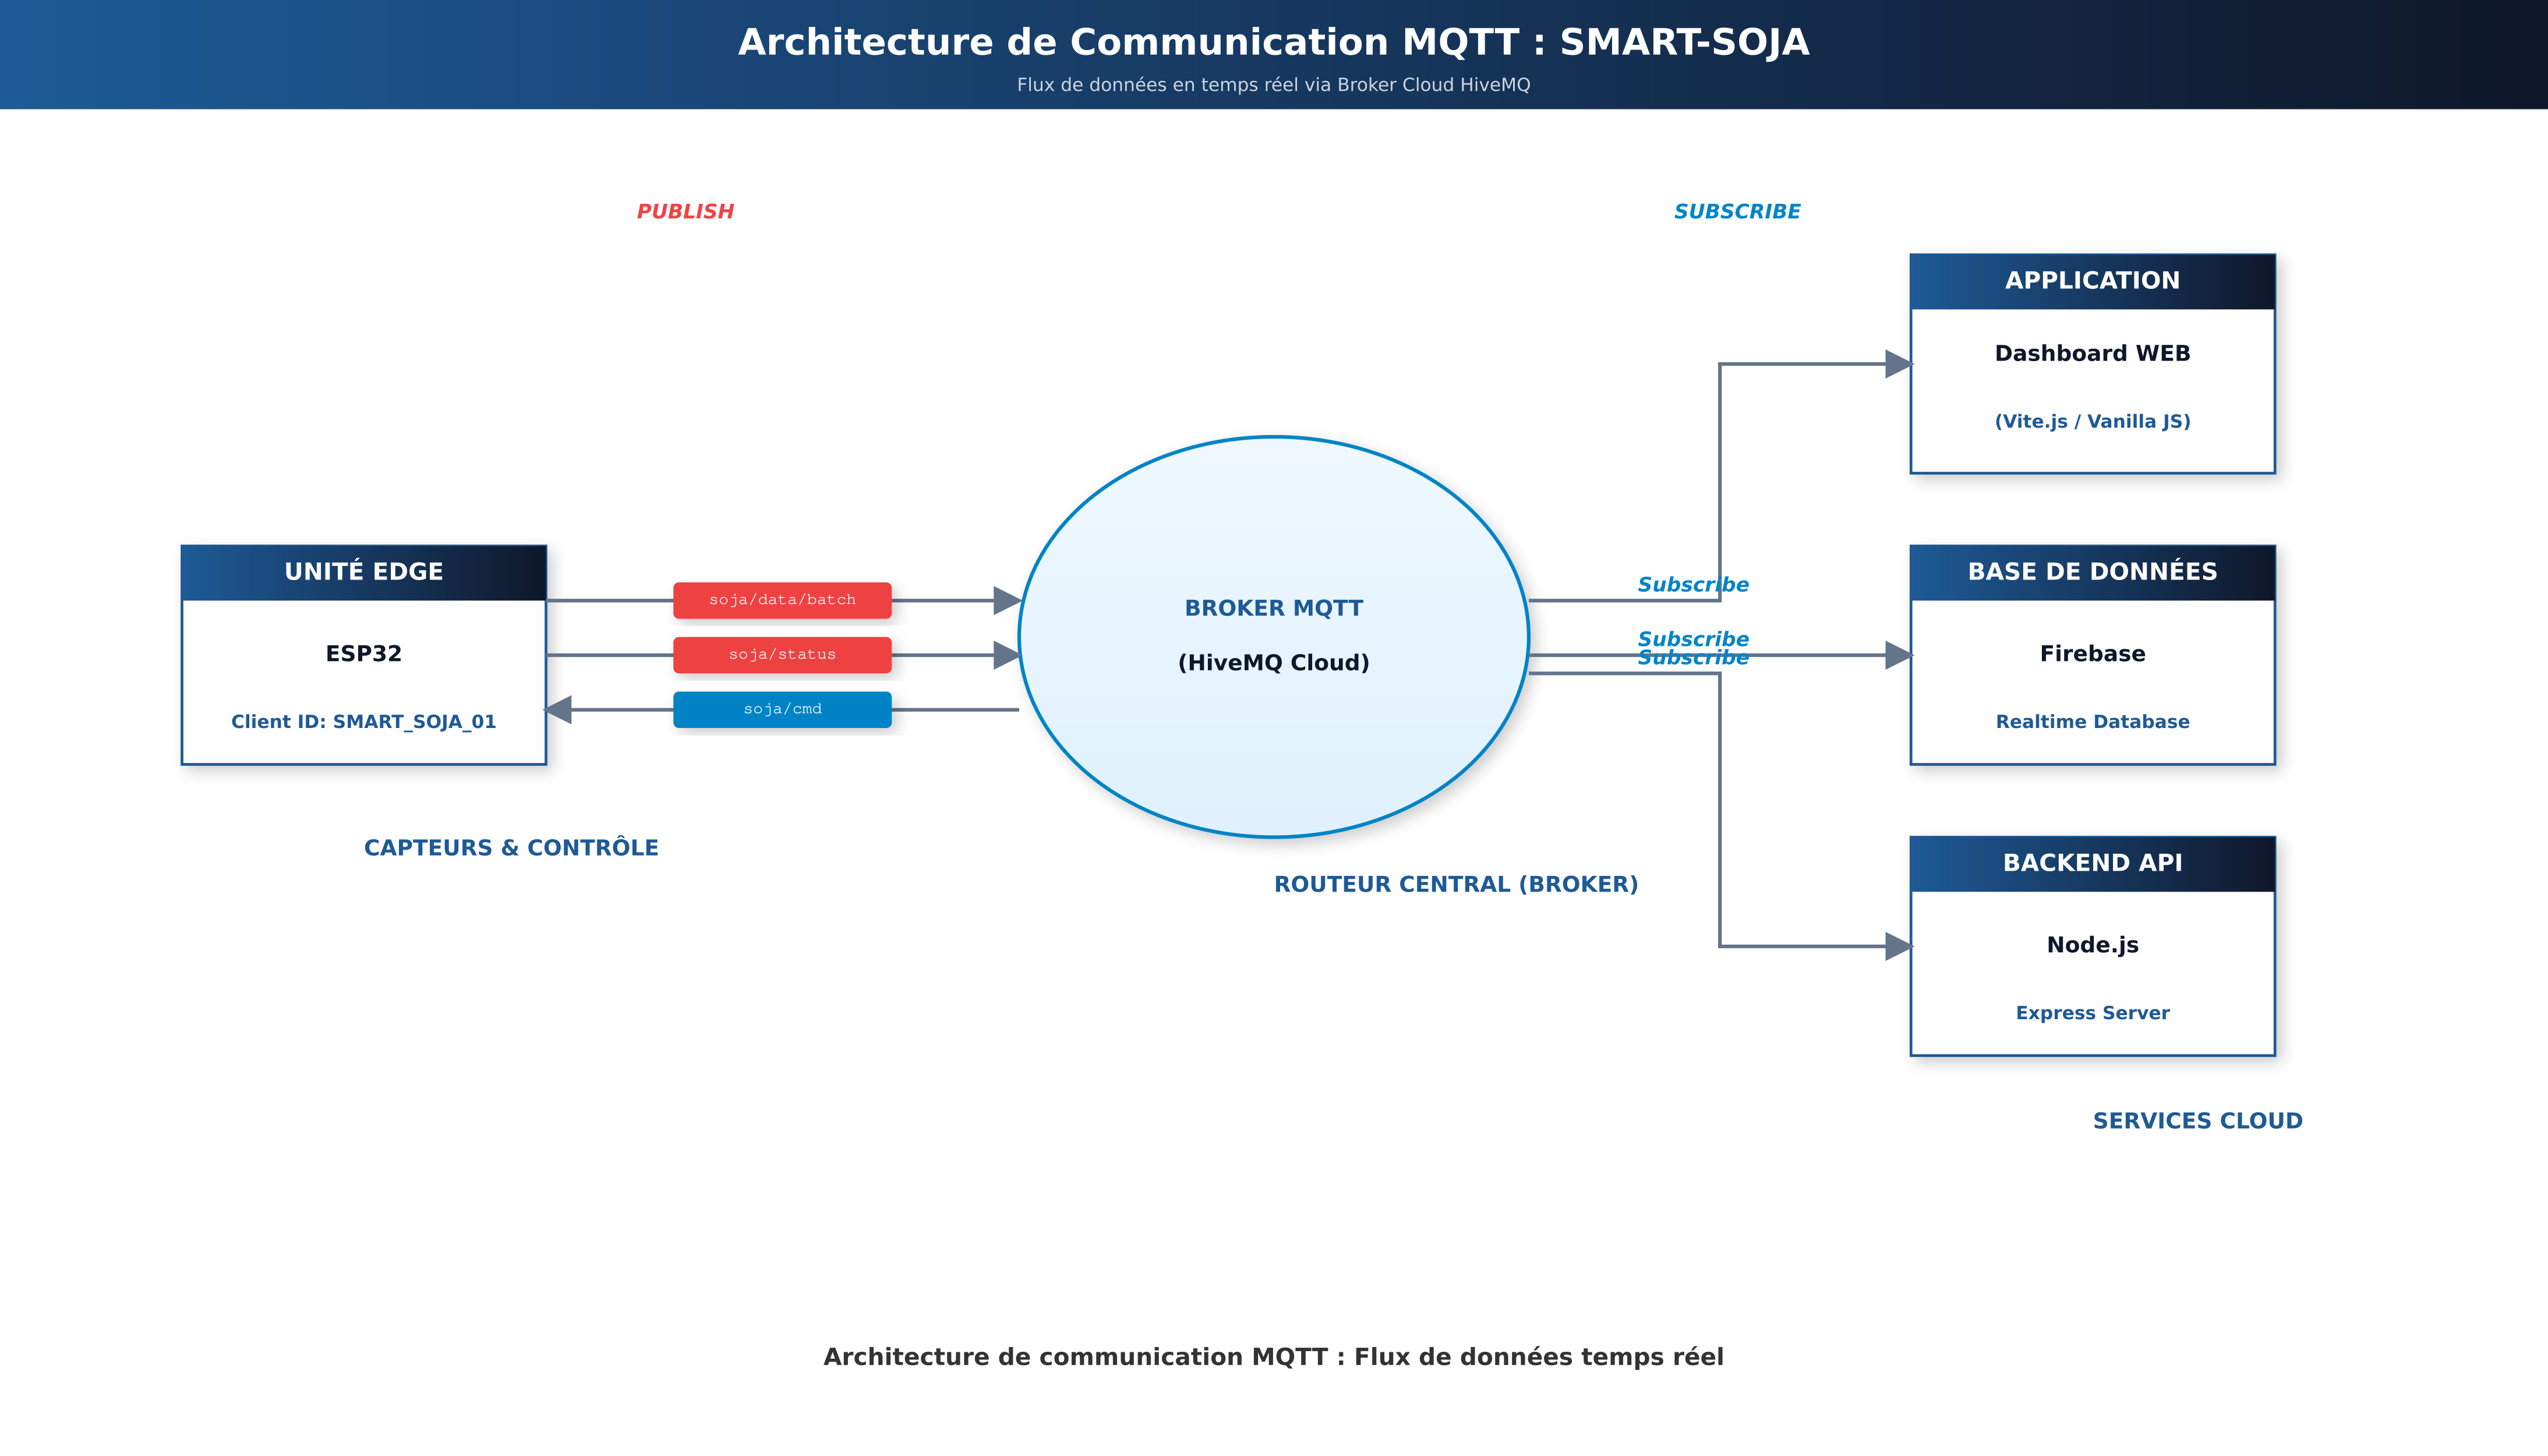
\includegraphics[width=\textwidth]{images/mqtt_architecture.png}
    \caption{Architecture de communication MQTT : Pipeline de données temps réel}
    \label{fig:diagram_mqtt}
\end{figure}
\FloatBarrier

Cette architecture garantit une \textbf{intégrité totale de la traçabilité} : chaque sac de soja possède son propre passeport numérique stocké de manière sécurisée dans le Cloud.

\begin{figure}[H]
    \centering
    \begin{subfigure}[b]{0.48\textwidth}
        \centering
        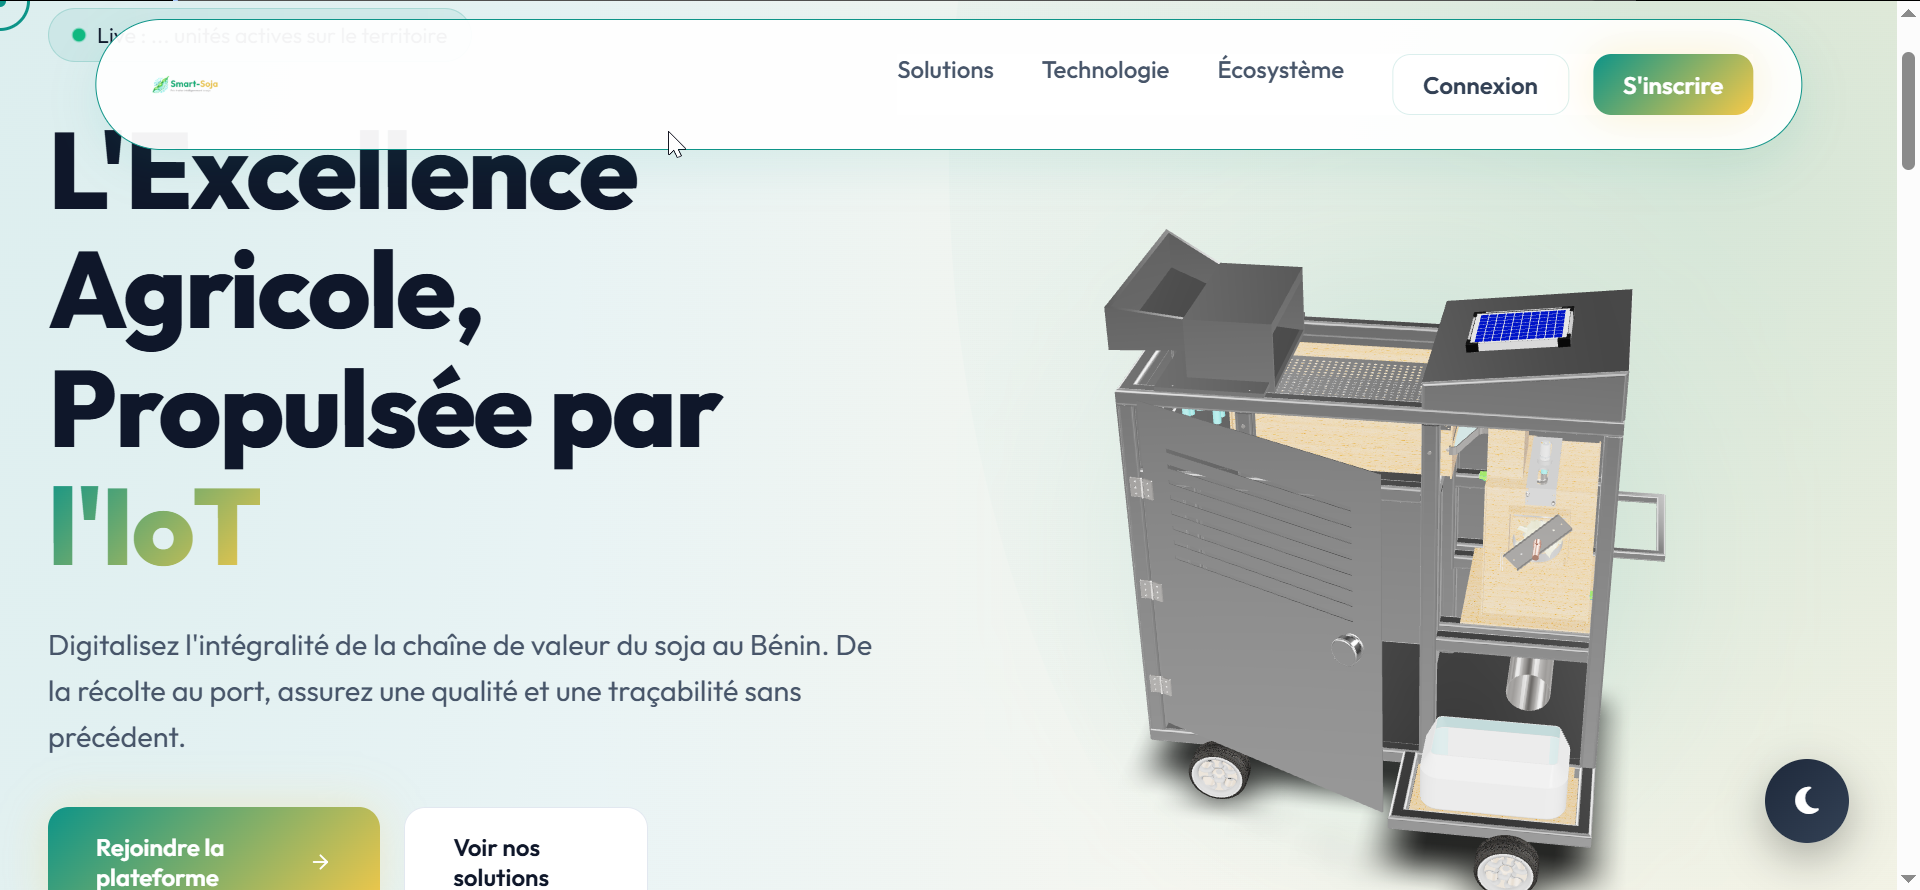
\includegraphics[width=\textwidth]{images/smart-soja-web_light.png}
        \caption{Mode Clair (\textit{Light Theme})}
    \end{subfigure}
    \hfill
    \begin{subfigure}[b]{0.48\textwidth}
        \centering
        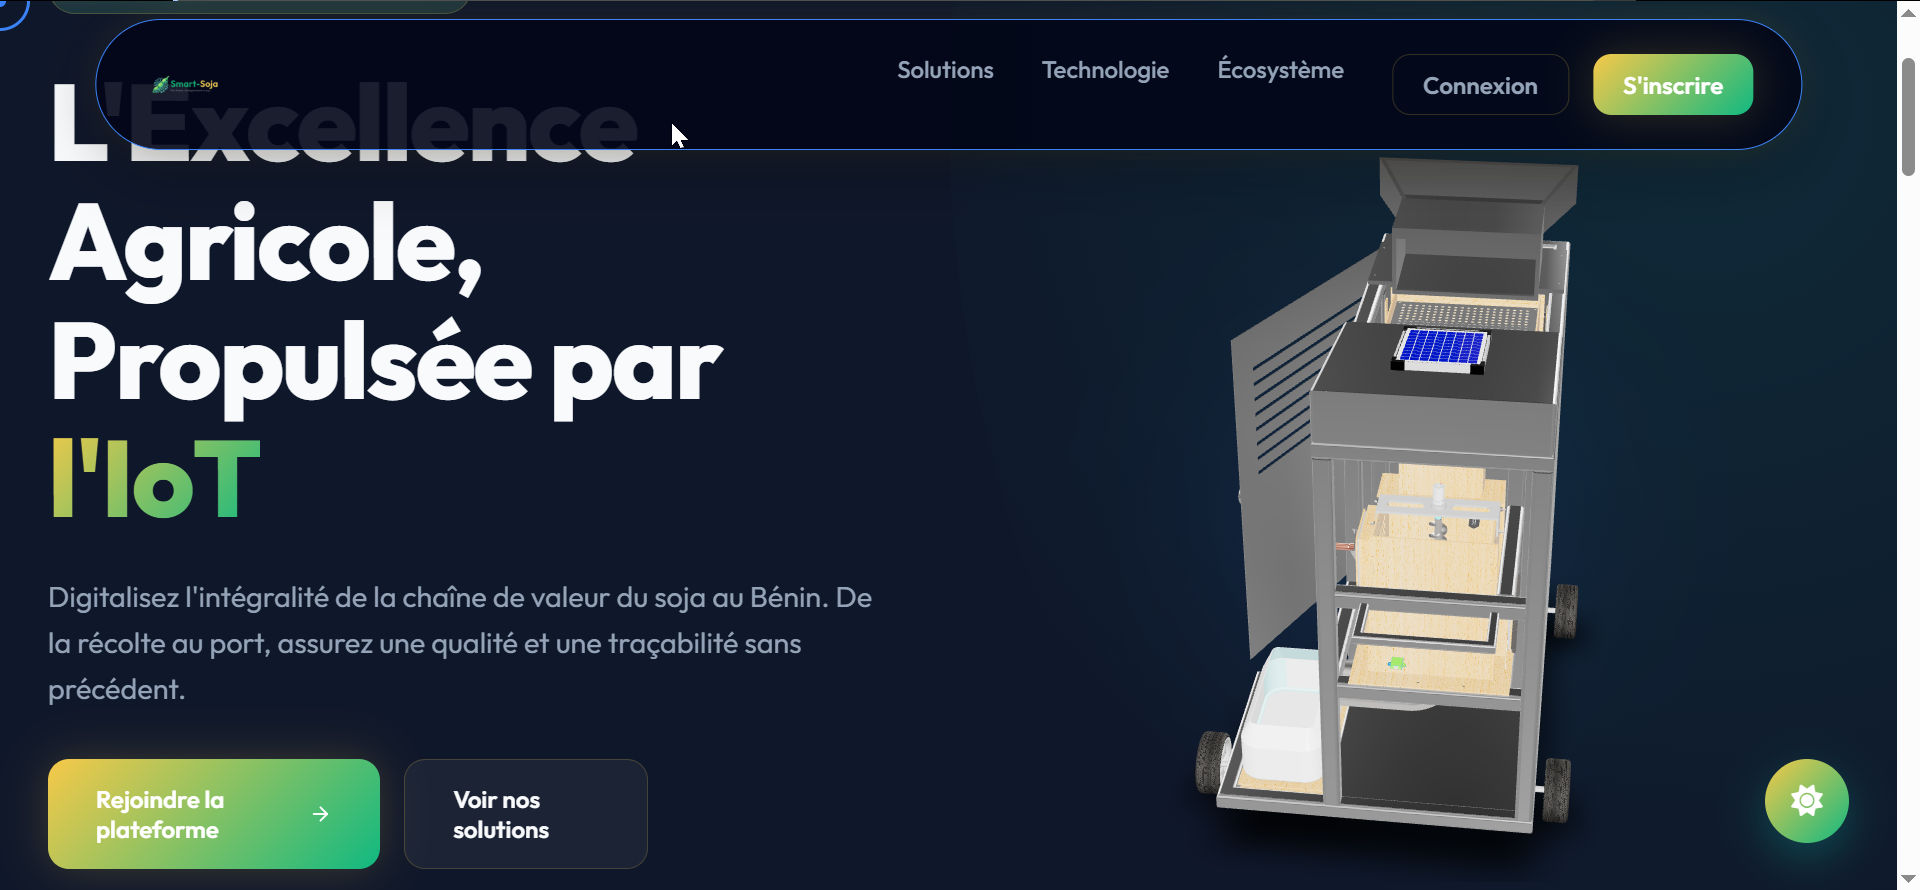
\includegraphics[width=\textwidth]{images/smart-soja-web_dark.png}
        \caption{Mode Sombre (\textit{Dark Theme})}
    \end{subfigure}
    \caption{Interface de présentation du projet SMART-SOJA — Page d'accueil (Vues multi-thèmes)}
    \label{fig:dashboard_themes}
\end{figure}
\FloatBarrier

Trois profils d'accès sont proposés :
\begin{itemize}
    \item \textbf{Tableau de bord Exploitant :} Suivi de production en temps réel, contrôle manuel des actionneurs via MQTT, alertes de maintenance.
    \item \textbf{Tableau de bord Industrie (GDIZ Ready) :} Validation de la qualité des lots entrants, graphiques d'humidité et température, impression des certificats de traçabilité PDF.
    \item \textbf{Tableau de bord Admin :} Gestion de la flotte de machines et des utilisateurs, audit système.
\end{itemize}

\FloatBarrier

% Fin de la section conception
